\documentclass{article}
\usepackage[left=1.5cm,top=2cm,right=1.5cm,bottom=2cm]{geometry}
\usepackage{fancybox}
\usepackage{fancyhdr}
\usepackage[brazil]{babel} 
\usepackage[dvipsnames]{xcolor}
\usepackage{tikz,pgfplots}
\pgfplotsset{compat=1.18}
\usetikzlibrary{calc,arrows}
\pagestyle{fancy}
\lhead{
\begin{tikzpicture}[overlay,remember picture]
\draw[draw=black] ($(current page.north west)
+ (1,-1)$) rectangle ($(current page.south east)+(-1,1)$);
\end{tikzpicture}

}
\chead{}
\rhead{}
\lfoot{}
\cfoot{}
\rfoot{}
\renewcommand{\headrulewidth}{0pt}

\usepackage[normalem]{ulem}
\usepackage{amsthm}
\usepackage{amsmath}
\usepackage{amsfonts}
\usepackage{amssymb}
\newcommand{\vs}{\vspace}
\newcommand{\hs}{\hspace}
\newcommand{\D}{\displaystyle}
\newcommand{\eq}{\begin{equation}}
\newcommand{\feq}{\end{equation}}
\usepackage{enumerate}
\usepackage{indentfirst}
\setlength{\parindent}{0.5cm}
\newcommand{\op}{\operatorname}
\usepackage{esvect}
\usepackage{upgreek}
\usepackage{graphicx}
\graphicspath{{figures/}}


\begin{document}
\begin{center}
    \textbf{\huge{Aplicação das equações de Lagrange}} 
    \\
    Leonardo Oliveira Gugé
\end{center}
Definimos a função de Lagrange (ou lagrangiana) $L$, que é,
por definição:
\begin{equation}
    L=T-V
\end{equation}
Onde $T$ é a energia cinética e $V$ é a energia 
potencial do sistema em questão.
Agora, as equações do movimento podem ser escritas na forma:
\begin{equation}
    \frac{d}{dt}(\frac{\partial L}{\partial \dot{q}_k})-
    \frac{\partial L}{\partial q_k}=0
\end{equation}
Vamos aplicar à máquina de Atwood:
\begin{center}
    
\begin{figure}[h]
    \centering
    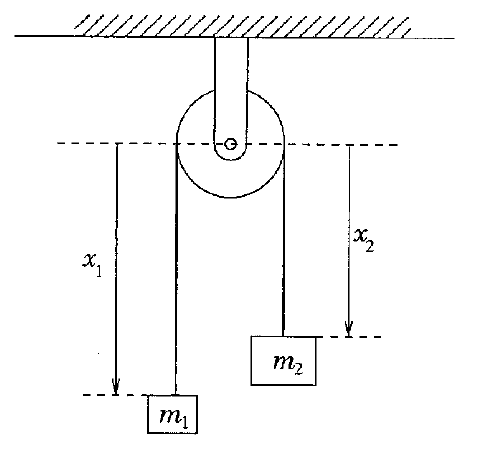
\includegraphics[scale=0.5]{Atwood}
    \caption{Máquina de Atwood}
\end{figure}

\end{center}
Primeiro, vamos determinar a lagrangiana desse sistema. Considerando
o nível zero do potencial gravitacional como sendo o plano horizontal
que passa pelo centro da polia, teremos então:
\begin{equation}
    V=-m_1g(l-x_1)-m_2g(l-x_2) 
\end{equation}
Nesse caso, consideramos $l$ determinada pelo raio da roldana e pelo
comprimento do fio, que supomos ser inextensível e de massa desprezível.
O vínculo que temos no sistema é:
\begin{equation}
    x_1+x_2=l
\end{equation}
Daí tiramos a condição de vínculo: $x_1+x_2=l$
donde $x_1=l-x_2$.
Logo, o potencial pode ser expresso por apenas uma das coordenadas
independentes(Nesse caso, $x_1$).
\begin{equation}
    V=-m_1g(l-x_1)-m_2gx_1
    \ \ \therefore \ \ 
    V=-m_1gl+m_1gx_1-m_2gx_1
\end{equation}
Para a energia cinética do sistema, faremos:
\begin{equation}
    T=\frac{m_1\dot{x_1}^{2}}{2} +\frac{m_2\dot{x_2}^{2}}{2}
\end{equation}
Pelas condições de vínculo:
\begin{equation}
    x_1+x_2=l \Rightarrow  \dot{x_1}+\dot{x_2}=0 \Rightarrow  \dot{x_1}=-\dot{x_2}
\end{equation}
Então, podemos reescrever a energia cinética do sistema como:
\begin{equation}
    T= \frac{m_1+m_2}{2}\dot{x_1}^{2}
\end{equation}
Agora, podemos calcular a lagrangiana $L$:
\begin{equation}
    L= \frac{m_1+m_2}{2}\dot{x_1}^{2} -m_1g(l-x_1)-m_2gx_2
\end{equation}

Aplicando as equações de Euler-Lagrange:
\begin{equation}
    \frac{d}{dt}(\frac{\partial L}{\partial \dot{x_1}})-
    \frac{\partial L}{\partial x_1}=0
\end{equation} 
\ \ \ Temos: 
\begin{equation}
    \frac{\partial L}{\partial \dot{x_1}}=(m_1+m_2)\dot{x_1} 
\end{equation}
\begin{equation}
    \frac{d}{dt}(\frac{\partial L}{\partial \dot{x_1}})=(m_1+m_2)\ddot{x_1}
\end{equation}
\begin{equation}
    \frac{\partial L}{\partial x_1}= m_1g-m_2g
\end{equation}
Portanto, a equação do movimento da máquina de Atwood para a coordenada $x_1$ é:
\begin{equation}
    (m_1+m_2)\ddot{x_1}-m_1g+m_2g=0
\end{equation}
Ou, simplismente:
\begin{equation}
    \ddot{x_1}=\frac{m_1-m_2}{m_1+m_2}g 
\end{equation}








\end{document}